%%%%%%%%%%%%%%%%%%%%%%%%%%%%%%%%%%%%%%%%%
% Beamer Presentation
% LaTeX Template
% Version 1.0 (10/11/12)
%
% This template has been downloaded from:
% http://www.LaTeXTemplates.com
%
% License:
% CC BY-NC-SA 3.0 (http://creativecommons.org/licenses/by-nc-sa/3.0/)
%
%%%%%%%%%%%%%%%%%%%%%%%%%%%%%%%%%%%%%%%%%

%----------------------------------------------------------------------------------------
%	PACKAGES AND THEMES
%----------------------------------------------------------------------------------------

\documentclass[handout]{beamer}

\mode<presentation> {

% The Beamer class comes with a number of default slide themes
% which change the colors and layouts of slides. Below this is a list
% of all the themes, uncomment each in turn to see what they look like.

%\usetheme{default}
%\usetheme{AnnArbor}
%\usetheme{Antibes}
%\usetheme{Bergen}
%\usetheme{Berkeley}
%\usetheme{Berlin}
%\usetheme{Boadilla}
%\usetheme{CambridgeUS}
%\usetheme{Copenhagen}
%\usetheme{Darmstadt}
%\usetheme{Dresden}
%\usetheme{Frankfurt}
%\usetheme{Goettingen}
%\usetheme{Hannover}
%\usetheme{Ilmenau}
%\usetheme{JuanLesPins}
%\usetheme{Luebeck}
\usetheme{Madrid}
%\usetheme{Malmoe}
%\usetheme{Marburg}
%\usetheme{Montpellier}
%\usetheme{PaloAlto}
%\usetheme{Pittsburgh}
%\usetheme{Rochester}
%\usetheme{Singapore}
%\usetheme{Szeged}
%\usetheme{Warsaw}

% As well as themes, the Beamer class has a number of color themes
% for any slide theme. Uncomment each of these in turn to see how it
% changes the colors of your current slide theme.

%\usecolortheme{albatross}
%\usecolortheme{beaver}
%\usecolortheme{beetle}
%\usecolortheme{crane}
%\usecolortheme{dolphin}
%\usecolortheme{dove}
%\usecolortheme{fly}
%\usecolortheme{lily}
%\usecolortheme{orchid}
%\usecolortheme{rose}
%\usecolortheme{seagull}
%\usecolortheme{seahorse}
%\usecolortheme{whale}
%\usecolortheme{wolverine}

%\setbeamertemplate{footline} % To remove the footer line in all slides uncomment this line
%\setbeamertemplate{footline}[page number] % To replace the footer line in all slides with a simple slide count uncomment this line

%\setbeamertemplate{navigation symbols}{} % To remove the navigation symbols from the bottom of all slides uncomment this line
}

\usepackage{graphicx} % Allows including images
\usepackage{booktabs} % Allows the use of \toprule, \midrule and \bottomrule in tables
\usepackage{cool}
\usepackage{tikz}
\usepackage{amsmath}
\DeclareMathOperator*{\argmax}{argmax}
\DeclareMathOperator*{\argmin}{argmin}
\usetikzlibrary{positioning}

%----------------------------------------------------------------------------------------
%	TITLE PAGE
%----------------------------------------------------------------------------------------

\title[HJB and Merton Portfolio]{HJB Equation and Merton's Portfolio Problem} % The short title appears at the bottom of every slide, the full title is only on the title page

\author{Ashwin Rao} % Your name
\institute[Stanford] % Your institution as it will appear on the bottom of every slide, may be shorthand to save space
{
ICME, Stanford University
 % Your institution for the title page
}

\date{\today} % Date, can be changed to a custom date

\begin{document}
\begin{frame}
\titlepage % Print the title page as the first slide
\end{frame}

\begin{frame}
\frametitle{Overview} % Table of contents slide, comment this block out to remove it
\tableofcontents % Throughout your presentation, if you choose to use \section{} and \subsection{} commands, these will automatically be printed on this slide as an overview of your presentation
\end{frame}

\section{Problem Statement}

\begin{frame}
\frametitle{Informal Problem Statement}
\pause
\begin{itemize}[<+->]
\item You will live for (deterministic) $T$ more years
\item Current Wealth + PV of Future Income (less Debt) is $W_0 > 0$.
\item You can invest in (allocate to) $n$ risky assets and a riskless asset
\item Each asset has known normal distribution of returns
\item Allowed to long or short any fractional quantities of assets
\item Trading in continuous time $0 \leq t < T$, with no transaction costs
\item You can consume any fractional amount of wealth at any time
\item Dynamic Decision: Optimal Allocation and Consumption at each time
\item To maximize lifetime-aggregated utility of consumption
\item Consumption Utility assumed to have constant Relative Risk-Aversion
\end{itemize}
\end{frame}

\begin{frame}
\frametitle{Problem Notation}
For simplicity, we state and solve the problem for 1 risky asset but the solution generalizes easily to $n$ risky assets.
\pause
\begin{itemize}[<+->]
\item Riskless asset: $dR_t = r \cdot R_t \cdot dt$
\item Risky asset: $dS_t = \mu \cdot S_t \cdot dt + \sigma \cdot S_t \cdot dz_t$ (i.e. Geometric Brownian)
\item $\mu > r > 0, \sigma > 0$ (for $n$ assets, we work with a covariance matrix)
\item Wealth at time $t$ is denoted by $W_t > 0$
\item Fraction of wealth allocated to risky asset denoted by $\pi(t, W_t)$
\item Fraction of wealth in riskless asset will then be $1 - \pi(t, W_t)$
\item Wealth consumption per unit time denoted by $c(t, W_t) \geq 0$
\item Utility of Consumption function $U(x) = \frac {x^{1-\gamma}} {1 - \gamma}$ for $0 < \gamma \neq 1$
\item Utility of Consumption function $U(x) = \log(x)$ for $\gamma = 1$
\item $\gamma =$ (constant) Relative Risk-Aversion $\frac {-x \cdot U''(x)} {U'(x)}$
\end{itemize}
\end{frame}

\begin{frame}
\frametitle{Problem Statement}
\pause
\begin{itemize}[<+->]
\item We write $\pi_t, c_t$ instead of $\pi(t, W_t), c(t, W_t)$ to lighten notation
\item Balance constraint implies the following process for Wealth $W_t$
$$dW_t = ((\pi_t \cdot (\mu - r) + r) \cdot W_t - c_t) \cdot dt + \pi_t \cdot \sigma \cdot W_t \cdot dz_t$$
\item At any time $t$, determine optimal $[\pi(t,W_t), c(t, W_t)]$ to maximize:
$$E[\int_t^T \frac {e^{-\rho (s-t)} \cdot c_s^{1-\gamma}} {1-\gamma} \cdot ds + \frac {e^{-\rho (T-t)} \cdot B(T) \cdot W_T^{1-\gamma}} {1-\gamma} \mid W_t]$$
\item where $\rho \geq 0$ is the utility discount rate, $B(T)$ is the bequest function
\item We can solve this problem for arbitrary bequest $B(T)$ but for simplicity, will consider $B(T) = \epsilon^{\gamma}$
where $0 < \epsilon \ll 1$, meaning ``no bequest'' (we need this $\epsilon$-formulation for technical reasons).
\item We will solve this problem for $\gamma \neq 1$ ($\gamma = 1$ is easier, hence omitted)
\end{itemize}
\end{frame}

\begin{frame}
\frametitle{Continuous-Time Stochastic Control}
\pause
\begin{itemize}[<+->]
\item Think of this as a continuous-time Stochastic Control problem
\item The {\em State} is $(t, W_t)$
\item The {\em Action} is $[\pi_t, c_t]$
\item The {\em Reward} per unit time is $U(c_t)$ 
\item The {\em Return} is the usual accumulated discounted {\em Reward}
\item Find {\em Policy} $: (t, W_t) \rightarrow [\pi_t, c_t]$ that maximizes the {\em Expected Return}
\item Note: $c_t \geq 0$, but $\pi_t$ is unconstrained
\end{itemize}
\end{frame}

\section{HJB Equation as Optimal Discounted Value Function PDE}

\begin{frame}
\frametitle{Optimal Discounted Value Function}
\pause
\begin{itemize}[<+->]
\item Instead of the usual Value Function ({\em Expected Return} from a given {\em State}), we consider the Discounted Value Function
\item Discounted Value Function is simply the Value Function further discounted to time 0
\item We focus on the Optimal Discounted Value Function $V^*(t, W_t)$
$$V^*(t, W_t) = \max_{\pi_t, c_t} E[\int_t^T \frac {e^{-\rho s} \cdot c_s^{1-\gamma}}{1 - \gamma} \cdot ds + \frac {e^{-\rho T} \cdot \epsilon^{\gamma} \cdot W_T^{1-\gamma}} {1 - \gamma} ]$$
\item $V^*(t, W_t)$ satisfies a simple recursive formulation for $0 \leq t < t_1 < T$.
$$V^*(t, W_t) = \max_{\pi_t, c_t} E[V^*(t_1, W_{t_1}) + \int_t^{t_1} \frac {e^{-\rho s} \cdot c_s^{1-\gamma}} {1 - \gamma} \cdot ds]$$
\end{itemize}
\end{frame}

\begin{frame}
\frametitle{HJB Equation for Optimal Discounted Value Function}
\pause
Rewriting in stochastic differential form, we have the HJB formulation
$$\max_{\pi_t, c_t} E[dV^*(t, W_t) + \frac {e^{-\rho t} \cdot c_t^{1-\gamma}}{1 - \gamma} \cdot dt] = 0$$
\pause
Use Ito's Lemma on $dV^*$, remove the $dz_t$ term since it's a martingale, and divide throughout by $dt$ to produce the HJB Equation in PDE form:
$$\max_{\pi_t, c_t} [\pderiv{V^*}{t} + \pderiv{V^*}{W_t} ((\pi_t (\mu - r) + r)W_t  - c_t)+ \pderiv[2]{V^*}{W_t} \frac {\pi_t^2 \sigma^2 W_t^2} {2} + \frac { e^{-\rho t} \cdot c_t^{1-\gamma}}{1 - \gamma}] = 0$$
\pause
Let us write the above equation more succinctly as:
$$\max_{\pi_t, c_t} \Phi(t, W_t; \pi_t, c_t) = 0$$
\pause
Note: we are working with the constraints $W_t > 0, c_t \geq 0$ for $0 \leq t < T$
\end{frame}

\begin{frame}
\frametitle{Optimal Allocation and Consumption}
Find optimal $\pi_t^*, c_t^*$ by taking partial derivatives of $\Phi(t, W_t; \pi_t, c_t)$ with respect to $\pi_t$ and $c_t$, and equate to 0 (first-order conditions for $\Phi$).
\pause
\begin{itemize}[<+->]
\item Partial derivative of $\Phi$ with respect to $\pi_t$:
$$(\mu -r) \cdot \pderiv{V^*}{W_t} + \pderiv[2]{V^*}{W_t} \cdot \pi_t \cdot \sigma^2 \cdot W_t = 0$$
$$ \Rightarrow \pi_t^* = \frac {-\pderiv{V^*}{W_t} \cdot (\mu - r)} {\pderiv[2]{V^*}{W_t} \cdot \sigma^2 \cdot W_t}$$
\item Partial derivative of $\Phi$ with respect to $c_t$:
$$-\pderiv{V^*}{W_t} + e^{-\rho t} \cdot (c_t^*)^{-\gamma} = 0$$
$$ \Rightarrow c_t^* = (\pderiv{V^*}{W_t} \cdot e^{\rho t})^{\frac {-1} {\gamma}}$$
\end{itemize}
\end{frame}

\begin{frame}
\frametitle{Optimal Discounted Value Function PDE}
\pause
Now substitute $\pi_t^*$ and $c_t^*$ in $\Phi(t, W_t; \pi_t, c_t)$ and set it to 0, which gets us the Optimal Discounted Value Function PDE:
\pause
$$\pderiv{V^*}{t} - \frac {(\mu - r)^2}{2 \sigma^2} \cdot \frac {(\pderiv{V^*}{W_t})^2} {\pderiv[2]{V^*}{W_t}}  + \pderiv{V^*}{W_t} \cdot r \cdot W_t + \frac {\gamma} {1 - \gamma} \cdot e^{\frac {-\rho t}{\gamma}} \cdot (\pderiv{V^*}{W_t})^{\frac {\gamma-1} {\gamma}} = 0$$ 
\pause
The boundary condition is:
$$V^*(T, W_T) = e^{-\rho T} \cdot \epsilon^{\gamma} \cdot \frac {W_T^{1-\gamma}} {1- \gamma}$$
\pause
The second-order conditions for $\Phi$ are satisfied {\bf under the assumptions} $c^*_t > 0, W_t > 0, \pderiv[2]{V^*}{W_t} < 0$ for all $0 \leq t < T$ (we will later show that these are all satisfied in the solution we derive), and for concave $U(\cdot)$, i.e., $\gamma > 0$
\end{frame}

\section{Reducing the PDE to an ODE}

\begin{frame}
\frametitle{Solving the PDE with a guess solution}
\pause
We surmise with a guess solution
$$V^*(t, W_t) = f(t)^{\gamma} \cdot e^{-\rho t} \cdot \frac {W_t^{1-\gamma}} {1-\gamma}$$
\pause
Then,
$$\pderiv{V^*}{t} = (\gamma \cdot f(t)^{\gamma-1} \cdot f'(t) -\rho \cdot f(t)^{\gamma}) \cdot e^{-\rho t} \cdot \frac {W_t^{1-\gamma}} {1-\gamma}$$
\pause
$$\pderiv{V^*}{W_t} = f(t)^{\gamma} \cdot e^{-\rho t} \cdot W_t^{-\gamma}$$
\pause
$$\pderiv[2]{V^*}{W_t} = - f(t)^{\gamma} \cdot e^{-\rho t} \cdot \gamma \cdot W_t^{-\gamma-1}$$
\end{frame}

\begin{frame}
\frametitle{PDE reduced to an ODE}
\pause
Substituting the guess solution in the PDE, we get the simple ODE:
$$f'(t) = \nu \cdot f(t) - 1$$
\pause
where $$\nu = \frac {\rho - (1 - \gamma) \cdot (\frac {(\mu - r)^2} {2 \sigma^2 \gamma} + r)} {\gamma}$$
\pause
with boundary condition $f(T) = \epsilon$.
\pause
\linebreak
The solution to this ODE is:
$$
f(t) =
\begin{cases}
\frac {1 + (\nu \epsilon - 1) \cdot e^{-\nu (T-t)}} {\nu} & \text{for } \nu \neq 0 \\
T-t+\epsilon & \text{for } \nu = 0 \\
\end{cases}
$$
\end{frame}

\section{Optimal Allocation and Consumption}
\begin{frame}
\frametitle{Optimal Allocation and Consumption}
\pause
Putting it all together (substituting the solution for $f(t)$), we get:
$$\pi^*(t, W_t) = \frac {\mu - r} {\sigma^2 \gamma}$$
\pause
$$
c^*(t, W_t)= \frac {W_t} {f(t)} = 
\begin{cases}
\frac {\nu \cdot W_t} {1 + (\nu \epsilon - 1) \cdot e^{-\nu (T-t)}} & \text{for } \nu \neq 0\\
\frac {W_t} {T-t+\epsilon} & \text{for } \nu = 0\\
\end{cases}
$$
\pause
$$
V^*(t, W_t) = 
\begin{cases}
e^{-\rho t} \cdot \frac {(1 + (\nu \epsilon - 1) \cdot e^{-\nu (T-t)})^{\gamma}} {\nu^{\gamma}} \cdot \frac {W_t^{1-\gamma}} {1-\gamma} & \text{for } \nu \neq 0\\
e^{-\rho t} \cdot \frac {(T-t+\epsilon)^\gamma \cdot W_t^{1 - \gamma}} {1-\gamma} & \text{for } \nu = 0\\
\end{cases}
$$
\pause
\begin{itemize}[<+->]
\item $f(t) > 0$ for all $0 \leq t < T$ (for all $\nu$) ensures $W_t, c^*_t > 0, \pderiv[2]{V^*}{W_t} < 0$. This ensures the constraints $W_t > 0$ and $c_t \geq 0$ are satisfied and the second-order conditions for $\Phi$ are also satisfied.
\item The HJB Formulation was key and this solution approach provides a template for similar continuous-time stochastic control problems.
\end{itemize}
\end{frame}

\section{Insights and Real-World Adaptation}

\begin{frame}
\frametitle{Gaining Insights into the Solution}
\pause
\begin{itemize}[<+->]
\item Optimal Allocation $\pi^*(t, W_t)$ is constant (independent of $t$ and $W_t$)
\item Optimal Fractional Consumption $\frac {c^*(t, W_t)} {W_t}$ depends only on $t$ ($=\frac 1 {f(t)}$)
\item With Optimal Allocation \& Consumption, the Wealth process is:
$$\frac {dW_t} {W_t} = (r + \frac {(\mu - r)^2} {\sigma^2 \gamma} - \frac 1 {f(t)}) \cdot dt + \frac {\mu - r} {\sigma \gamma} \cdot dz_t$$
\item Expected Portfolio Return is constant over time ($=r + \frac {(\mu - r)^2} {\sigma^2 \gamma}$)
\item Assuming $\epsilon < \frac 1 {\nu}$, Fractional Consumption $\frac 1 {f(t)}$ increases over time
\item Expected Rate of Wealth Growth $r + \frac {(\mu - r)^2} {\sigma^2 \gamma} - \frac 1 {f(t)}$ decreases over time
\item If $r + \frac {(\mu - r)^2} {\sigma^2 \gamma} > \frac 1 {f(0)}$, we start by Consuming $<$ Expected Portfolio Growth and over time, we Consume $>$ Expected Portfolio Growth
\item Wealth Growth Volatility is constant ($= \frac {\mu - r} {\sigma \gamma}$)
\end{itemize}

\end{frame}

\begin{frame}
\frametitle{Portfolio Return versus Consumption Rate}
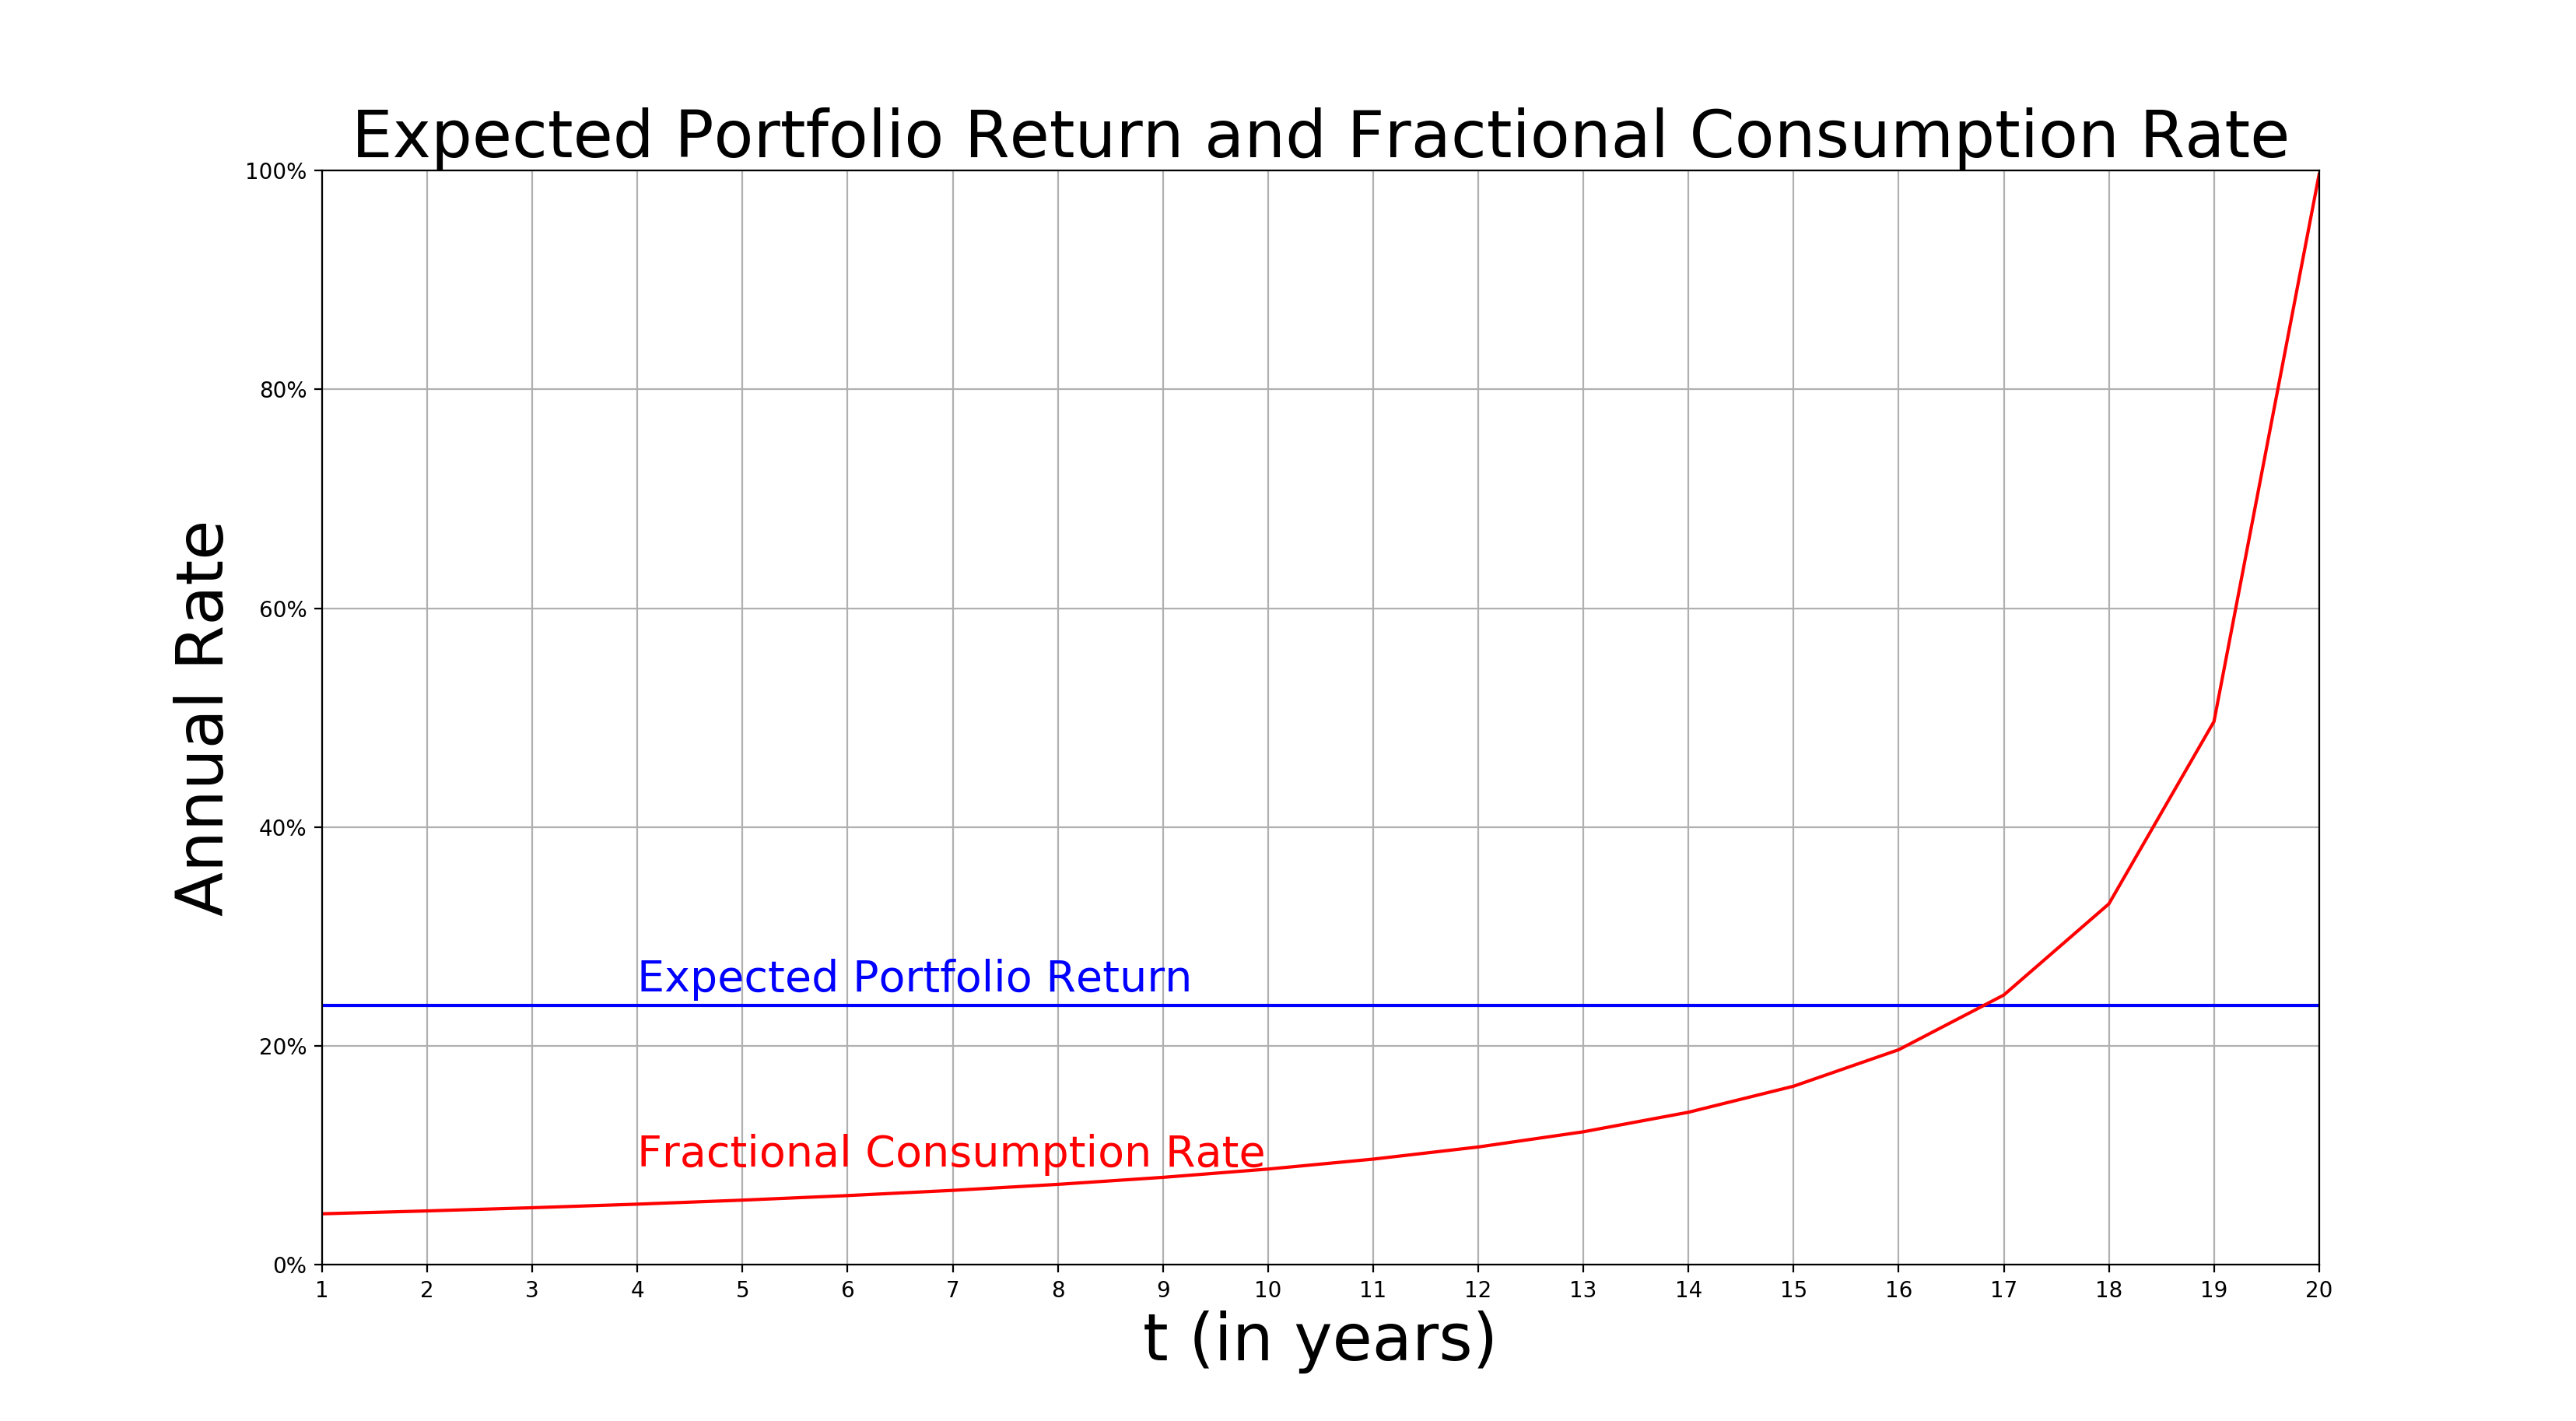
\includegraphics[width=12cm, height=8cm]{portfolio.png}
\end{frame}

\begin{frame}
\frametitle{Porting this to Real-World Portfolio Optimization}
\pause
\begin{itemize}[<+->]
\item Analytical tractability in Merton's formulation was due to:
\begin{itemize}
\item Normal distribution of asset returns
\item Constant Relative Risk-Aversion
\item Frictionless, continuous trading
\end{itemize}
\item However, real-world situation involves:
\begin{itemize}
\item Discrete amounts of assets to hold and discrete quantities of trades
\item Transaction costs
\item Locked-out days for trading
\item Non-stationary/arbitrary/correlated processes of multiple assets
\item Changing/uncertain risk-free rate
\item Consumption constraints
\item Arbitrary Risk-Aversion/Utility specification
\end{itemize}
\item $\Rightarrow$ Approximate Dynamic Programming or Reinforcement Learning
\item Large Action Space points to Policy Gradient Algorithms
\end{itemize}
\end{frame}

\end{document}